\section{Motiva��o}

\subsection{Motiva��o}

\begin{frame}\frametitle{Motiva��o} 
\begin{itemize}
	\item Atualmente, h� uma necessidade de se criar modelos 3D cada vez maiores e com grande n�vel de detalhe.
	\item Por�m, quanto maior e mais detalhado o modelo, mais tempo ter� que ser gasto por um modelador para faz�-lo.
	\item A� entra a gera��o procedural...
\end{itemize}	
\end{frame}

\subsection{Gera��o Procedural}

\begin{frame}\frametitle{O que � gera��o procedural?} 
\begin{itemize}
	\item Gera��o procedural � um termo gen�rico para descrever algoritmos que determinam caracter�sticas de efeitos ou modelos.
	\item Vantagens:
	\begin{itemize}
		\item Flexibilidade: alterando os par�metros do algoritmo, � poss�vel gerar um grande n�mero de modelos.
		\item Espa�o: n�o h� necessidade de um grande espa�o em disco, j� que tudo ser� ditado por algoritmos.
	\end{itemize}
\end{itemize}
\end{frame}


%\begin{frame}\frametitle{Gera��o Procedural X Entradas do Usu�rio}
%\begin{itemize}
%	\item Quanto menor o n�mero de entradas do usu�rio, maior o n�vel de gera��o procedural.
%\end{itemize}
%\begin{center}
%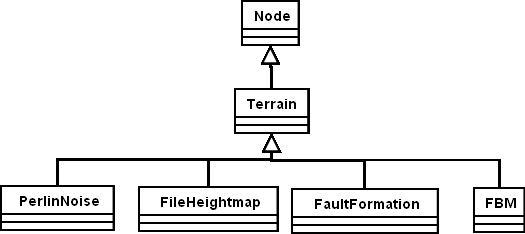
\includegraphics[width=0.5\linewidth]{img/node}
%\end{center}
%\end{frame}



%\begin{frame}\frametitle{Exemplos}
%\begin{columns}
%	\begin{column}{5cm}
%	\begin{itemize}
%		\item \alert<1>{.kkrieger\\} \only<1>{\scriptsize Praticamente tudo gerado proceduralmente}
%		\item \alert<2>{Elite (1984)\\} \only<2>{\scriptsize Oito gal�xias, 256 planetas.}
%		\item \alert<3>{SpeedTree\\} \only<3>{\scriptsize �rvores geradas proceduralmente.}
%	\end{itemize}
%	\vspace{3cm} 
%	\end{column}
%	\begin{column}{5cm}
%	\begin{overprint}
%		\includegraphics<1>[width=1.0\linewidth]{img/kkrieger}
%		\includegraphics<2>[width=1.0\linewidth]{img/elite}
%		\includegraphics<3>[width=1.0\linewidth]{img/speedtree}
%	\end{overprint}
%	\end{column}
%\end{columns}
%\end{frame}

\begin{frame}\frametitle{GPU} 
\begin{itemize}
	\item As atuais placas de v�deo possuem \emph{GPUs} com milhares de unidades de processamento.
	\item Constru�das de forma a processar da melhor maneira poss�vel um grande n�mero de dados independentes entre si, como � o caso de v�rtices e \emph{pixels}.
\end{itemize}
\begin{center}
	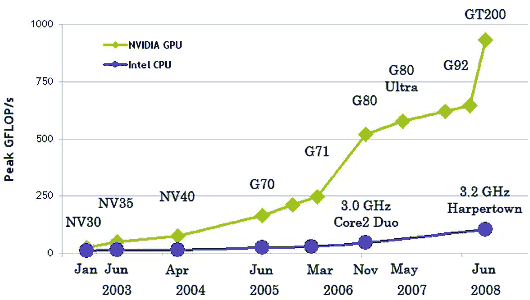
\includegraphics[width=0.5\linewidth]{img/gflops}
\end{center}
\end{frame}

